% main.tex
\documentclass[12pt]{article}

\usepackage[margin=1in]{geometry}
\usepackage{natbib}
\usepackage{hyperref}
\hypersetup{
  colorlinks=true,
  linkcolor=blue,
  filecolor=magenta,
  citecolor=blue,
  urlcolor=cyan,
  pdftitle={How to Study Boundary Phenomena},
  pdfpagemode=FullScreen,
}
\usepackage[T1]{fontenc}
\usepackage[utf8]{inputenc}
\usepackage{amsmath}
\usepackage{graphicx}
\usepackage{tipa}

\title{Language as a Stack of Homeostatic Property-Cluster Kinds: From Phonemes to Constructions}
\author{Brett Reynolds}
\date{}

\begin{document}
\maketitle

\begin{abstract}
\noindent Categories in language are stable enough to support reliable inference yet flexible enough to drift, diversify, and admit exceptions. I argue that many linguistic categories---phonemes, lexemes, and language-internal constructions---are \textsc{homeostatic property-cluster} (HPC) kinds: probabilistic clusters of articulatory, acoustic, semantic, and distributional properties stabilized by identifiable mechanisms at biological, cognitive-developmental, and sociocultural levels. Building on Miller's account of words as HPCs, which rejects essence-based individuation in favor of mechanism-indexed clusters, and on recent evidence that phonemes function as culturally maintained cognitive tools, I generalize the HPC template across linguistic levels and supply operational diagnostics and compact case studies. The diagnostics are (i) a projectibility test: tokens of a proposed kind support out-of-sample inferences about form/meaning/distribution; and (ii) a homeostasis test: specific stabilizers can be named and their property covariance shown. I demonstrate these with (A) phoneme typology (inventory ridgelines by family and the probability of /y/ increasing with vowel-inventory size), (B) a word-level diachrony showing distributional ``cluster cohesion'' under semantic drift, and (C) an English construction (\textit{let alone}), with cue bundling and cross-corpus replication. I also delimit non-HPCs: one-off items (nonce coinages), analyst-level macro-categories (e.g., cross-linguistic ``resultative'' as a single kind), and negative/complement classes. The result is a general method for deciding when a linguistic category earns kindhood by HPC lights, why some categories travel well across speakers and time, and where category proposals fail. The approach integrates philosophy-of-science clarity about kinds with quantitative, reproducible analyses familiar to cognitive science \citep{Miller2021WordsSpeciesKinds,Ekstrom2025PhonemeTool}.
\end{abstract}

\section*{Outline}
\begin{enumerate}
  \item \textbf{Introduction:} Frame the problem of category stability without essences; motivate HPC kinds for language; preview diagnostics and contributions; position relative to \citet{Miller2021WordsSpeciesKinds} and the ``phoneme as cognitive tool'' results \citep{Ekstrom2025PhonemeTool}.
  \item \textbf{Framework and diagnostics:} Define HPC for linguistic categories; state projectibility and homeostasis tests; map stabilizers (biophysical, developmental, sociocultural) and show how they correspond to the cognitive-tool criteria.
  \item \textbf{Case A (phoneme, positive):} Replicate family-wise inventory ridgelines and model $P(\text{/y/}\mid \text{vowel-inventory size})$; interpret patterns as signatures of homeostasis (quantal regions, dispersion), with developmental and normative scaffolding.
  \item \textbf{Case B (word, positive under drift):} One lexeme with documented semantic change (distributional neighborhood cohesion across decades; held-out prediction) consistent with Miller's mechanism-first individuation of word-kinds.
  \item \textbf{Case C (construction, positive):} \textit{let alone} as an HPC: cue bundling, collostructional profiles, and cross-corpus replication; stabilize via frequency, redundancy, and local performance standards.
  \item \textbf{Failures:} Too thin (nonce items, performance blends), too fat (global ``resultative''/``ditransitive''), and negative/complement classes (``ungrammatical strings''); reserve kindhood for local equilibria.
  \item \textbf{Predictions and disconfirmers:} Perturbation and scaling predictions; what would falsify an HPC claim at each level.
  \item \textbf{General discussion:} What HPC buys cognitive science; limits and next steps (developmental evidence; iterated-learning models; cross-linguistic extension).
\end{enumerate}

\section{Introduction}
Language presents a familiar problem for cognitive science: the categories I rely on to speak and understand are stable enough to underwrite reliable inference yet flexible enough to drift and diversify. An attractive middle ground---originating in Boyd’s account of \textsc{homeostatic property–cluster} (HPC) kinds---treats many scientific and social categories as probabilistic clusters stabilized by mechanisms that keep enough of the cluster together for inductive use \citep{Boyd1991Enthusiasm,Boyd1999Homeostasis}\footnote{For the first explicit HPC formulation (applied to moral terms), see \citet[§3.8]{Boyd1988MoralRealist}. For an explicit allowance that social mechanisms can underwrite homeostasis, see \citet{Boyd2000Workmanship}.}. On that understanding, I treat phonemes, words, and language-internal constructions as a posteriori kinds maintained by identifiable stabilizers.

For words, \citet{Miller2021WordsSpeciesKinds} develops this stance, rejecting essence-based individuation in favor of mechanism-indexed clusters that are historically delimited and population-relative. On this view, word-kinds earn their status because internal (cognitive) and external (normative) mechanisms sustain covarying properties---pronunciation, orthography, meaning, distribution---so that speakers can project from attested tokens to new ones.


At the phonological level, recent work argues that phonemes are culturally maintained \textsc{cognitive tools} anchored in articulatory and auditory constraints. Two quantitative signatures exemplify the sort of measurable ``homeostasis'' HPC requires: family-wise \textsc{ridgelines} of inventory sizes showing most languages cluster roughly between 20 and 50 segments, and a scaling curve in which the probability that a language includes /y/ rises with vowel-inventory size, while /i/ remains common even in small systems. Both patterns are presented with explicit methodological detail and tied to biophysical and efficiency pressures, and a compact checklist of tool criteria summarizes the stabilizers involved \citep[Fig.\,1 p.\,4; Fig.\,2 p.\,7; Table\,1 p.\,14]{Ekstrom2025PhonemeTool}. These are precisely the ingredients HPC seeks: projectible distributions and identifiable stabilizing mechanisms.

This article proposes a general, testable program: many linguistic categories---phonemes, lexemes, and language-internal constructions---are HPC kinds. The claim is operational, not merely analogical. I introduce two diagnostics and apply them across levels with compact, reproducible case studies, alongside a principled failure taxonomy that blocks over-generalization.

Diagnostic 1: Projectibility. A proposed category is projectible if tokens support reliable out-of-sample inference about form, meaning, or distribution. This can be quantified with cross-corpus replication, held-out prediction, or cluster-cohesion under temporal or register shifts.

Diagnostic 2: Homeostasis. A proposed category is homeostatic if its property cluster can be tied to specific stabilizers---biophysical attractors (e.g., quantal stability, dispersion), acquisition dynamics (e.g., perceptual magnets; sensorimotor adaptation), and sociocultural norms (local performance standards; entrenchment)---and if the expected covariance among properties can be demonstrated.

The first case study revisits the phoneme level using PHOIBLE-derived summaries but focuses on signatures rather than re-deriving physiology: inventory ridgelines by family and a logistic model for $P(\text{/y/})$ given inventory size, with family-wise subsampling as a sensitivity check. The HPC reading is straightforward: projectibility follows from the tight family distributions; homeostasis is underwritten by quantal stability and dispersion, with developmental tuning and community norms supplying the cultural scaffolding \citep{Ekstrom2025PhonemeTool}.

The second case study turns to words. Building on \citet{Miller2021WordsSpeciesKinds}, I track distributional drift for a single lexeme undergoing semantic change and show that a distributional neighborhood remains cohesive enough for decade-held-out prediction. Projectibility is demonstrated empirically; homeostasis is attributed to entrenchment and norm-guided usage that keep orthography/phonology/meaning covarying at usable levels, even as meanings shift.

The third case study treats an English construction, \textit{let alone}, as a language-internal HPC kind. Its cue bundle (string anchor, syntactic environment, conventionalized pragmatic contrast) yields robust extraction and cross-corpus replication; stabilizers include frequency, redundancy of cues, and normative enforcement (including editorial practices). Projectibility is tested by training on one corpus and predicting on another.

Equally important are the failure cases. Some proposals are too thin: one-off items (nonce coinages), performance blends, and child-only overregularizations within the adult standard lack the stabilizers that make inference sensible. Others are too fat: analyst-level macro-categories such as cross-linguistic ``resultative'' or ``ditransitive'' pool distinct local equilibria; the relevant mechanisms are local, so the global umbrella is not a single HPC kind. Finally, negative or complement classes (e.g., ``ungrammatical strings'') are defined by failure rather than by a causally sustained cluster. The discipline here is mechanism-first, in line with the word-kinds program \citep{Miller2021WordsSpeciesKinds}.

The framework yields predictions and disconfirmers. A perturbation prediction: weakening a stabilizer (e.g., lowering frequency or impoverishing input) will reduce cluster covariance before norms re-stabilize---a pattern testable under register shifts or in learner corpora. A scaling prediction: rarer but quantally robust members (e.g., /y/ in the vowel space) become more probable as system size grows; analogously, low-frequency constructional variants should be more prevalent in larger constructicons. Both predictions borrow directly from the phoneme results \citep[Fig.\,2 p.\,7]{Ekstrom2025PhonemeTool} and extend them to higher levels.

In sum, properly operationalized HPC naturalizes linguistic ontology for cognitive science. It tells us when a category is the right sort of thing to underwrite inference, what keeps it stable enough, and how it can change. At the phoneme level, the ridgeline and scaling patterns already instantiate homeostasis under constraint; at the word and construction levels, analogous signatures can be demonstrated with standard corpus methods. The result is not that everything is an HPC, but that many linguistic categories pass a disciplined test---and some do not \citep{Miller2021WordsSpeciesKinds,Ekstrom2025PhonemeTool}.

\section{Framework and diagnostics}\label{sec:framework}

The claim that linguistic categories are HPC kinds is ontological in spirit but have to be cashed out operationally. On the Boydian view, kinds are a posteriori and population–time relative: they are groupings whose members share a family of properties tightly enough for inductive use because there are mechanisms that, in fact, keep enough of those properties together \citep{Boyd1991Enthusiasm,Boyd1999Homeostasis}. Boyd first articulates the \textsc{HPC} template for moral terms \citep[§3.8]{Boyd1988MoralRealist} and later makes explicit that social mechanisms can underwrite homeostasis as well \citep{Boyd2000Workmanship}. That is why the framework is a natural fit for language, where physical constraints, learning dynamics, and norms jointly shape categories.

Two diagnostic questions organize what follows. First, projectibility: does the proposed category support reliable out-of-sample inference? Here the touchstones are familiar to cognitive science. A category projects when held-out data behave like the data that fixed our expectations: ridge-like concentration of inventory sizes by family; cross-corpus replication of a construction’s cue bundle; decade-held-out prediction for a drifting lexeme. Projectibility is not a metaphysical add-on but the observable face of kindhood: if I can't predict beyond the training slice, talk of a kind is idle.

Second, homeostasis: are there identifiable mechanisms that would make the observed covariance non-accidental, and do I see their expected signatures? At the phoneme tier, articulatory–auditory attractors and dispersion pressures are the obvious candidates; at higher tiers, frequency-driven entrenchment, cue redundancy, acquisition trajectories, editorial and community norms do analogous work. The recent “phoneme as cognitive tool” synthesis is helpful here because it treats these mechanisms as a stack and shows what their fingerprints look like: a narrow band of inventory sizes across families, scaling of rarer vowels with system size, and learnability patterns that bind cues within categories \citep[Fig.\,1; Fig.\,2; Table~1]{Ekstrom2025PhonemeTool}. For words, Miller’s mechanism-first treatment makes the same point from another angle: kindhood turns on sustained covariation among orthography, phonology, meaning, and distribution in a population and time slice, not on essences \citep{Miller2021WordsSpeciesKinds}.

The protocol, then, is straightforward even when the representational commitments differ across theories. I begin by stating the properties in play for the proposed category and the stabilizers that plausibly couple them in the relevant population and period. I ask for projectibility in the mundane, empirical sense—held-out prediction or cross-corpus replication above reasonable baselines—and I look for the signatures the stabilizers predict: scaling relations rather than arbitrary curves, stability bands rather than scatter, cue bundling rather than brittle single cues, inertia under drift rather than whiplash. Where those pieces line up, I have warrant to treat the category as an \textsc{HPC} kind. Where they do not—where predictive grip disappears, where no credible stabilizer can be named, or where the purported signatures fail to materialize—I withhold the label.

Two guardrails prevent overreach. First, scope is local. Cross-linguistic umbrellas such as “resultative” or “ditransitive” pool heterogeneous mechanisms; they are interest-relative classifications rather than single kinds. The same reasoning pares back analyst-aggregated macro-families of constructions within a language when the stabilizers diverge. Second, negatives are not kinds. Complement classes (“the set of ungrammatical strings,” “exceptions to rule $R$”) and one-off items (nonce coinages, performance blends) lack a stabilizing base by design; they may be explananda, but not kinds in the relevant sense.

This framing keeps the metaphysics modest and the tests empirical. It does not presuppose a specific architecture of grammar or a commitment to categorical perception; it asks instead whether a putative linguistic category earns its keep by being predictively useful in virtue of mechanisms I can name and whose traces I can see. The next sections apply that discipline to phonemes, words, and one English construction, and mark the boundaries where \textsc{HPC} talk should stop.


\section{Case A—Phonemes: a positive HPC}\label{sec:case-phoneme}

The phoneme tier is the cleanest place to test the claim that linguistic categories are HPC kinds. Inventories are comparable across languages, there is independent theory about plausible stabilizers, and open resources allow a fully reproducible analysis. I use PHOIBLE~2.0 \citep{MoranEtAl2019PHOIBLE} to derive two complementary signatures: a family‐wise concentration of total inventory sizes and a scaling relation linking the probability of /y/ to vowel‐inventory size. On the \textsc{projectibility} side, the question is whether unseen languages behave like held‐out members of their families or like random draws from a diffuse space. On the \textsc{homeostasis} side, the question is whether known mechanisms—articulatory–auditory attractors, dispersion, learning dynamics, and sociocultural norms—are a credible basis for the observed covariance \citep{Stevens1989Quantal,LiljencrantsLindblom1972,Lindblom1990HandH,Ekstrom2025PhonemeTool}.

For each language I count distinct consonant and vowel segments, excluding tones and prosodic units; when PHOIBLE lists multiple inventories for the same language, I keep the largest and document the choice. Families follow Glottolog. Figure~\ref{fig:ridgelines} plots kernel–density ridgelines of total inventory sizes by family (families with fewer than ten languages are omitted; ordering is by family median). The picture is strikingly regular: medians cluster in a narrow band roughly between 20 and 50 segments, with thin tails beyond that range. Because densities are estimated independently by family, the shared band is not an artefact of pooling; it is a cross‐family regularity that licenses out‐of‐sample expectations for new languages in known families. The pattern matches typological summaries and aligns with the cognitive-tool review \citep[Fig.\,1]{Ekstrom2025PhonemeTool}.

% --- Figure: Inventory ridgelines by family ---
\begin{figure}[t]
  \centering
  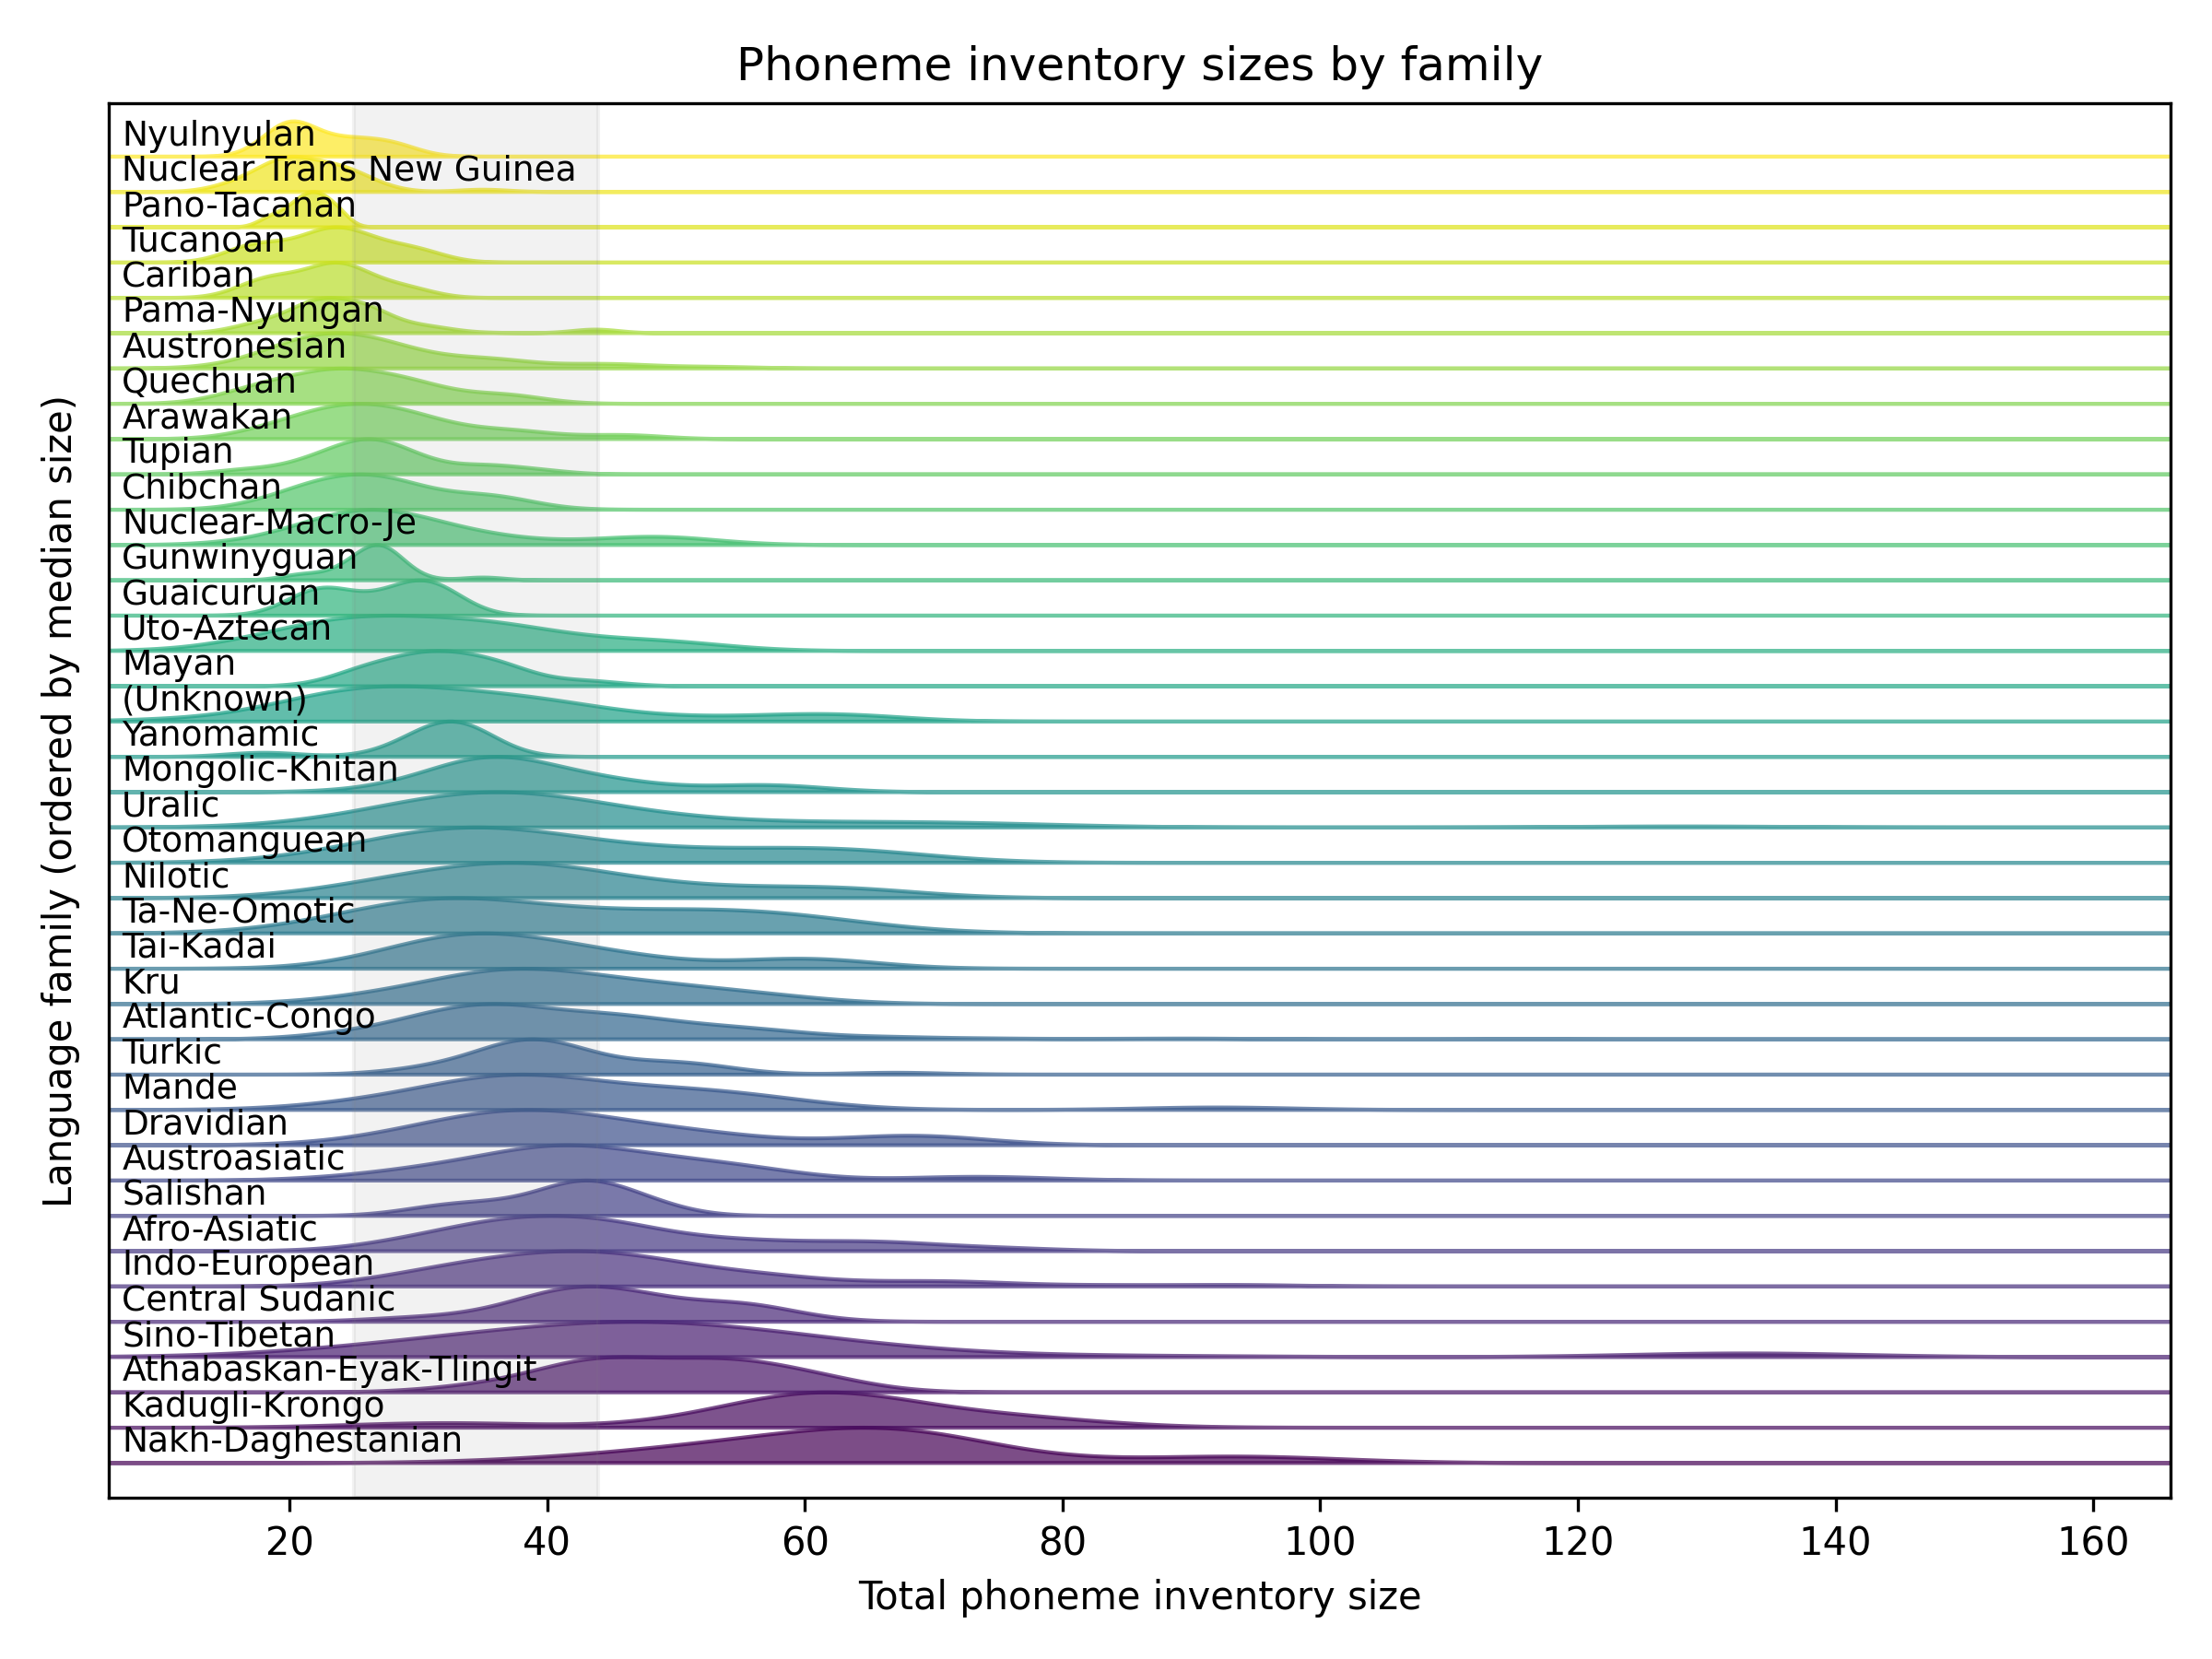
\includegraphics[width=\linewidth]{images/inventory_ridgelines.png}
  \caption{Phoneme inventory sizes by language family (PHOIBLE~2.0).
  Densities are shown for families with $n \ge 10$ languages, ordered by family median.
  Most families cluster in the 20–50 range (shaded), consistent with a homeostatic regime under articulatory–perceptual and dispersion constraints.
  Data: PHOIBLE~2.0; analysis code and exact processing steps are provided in the companion repository.}
  \label{fig:ridgelines}
\end{figure}

The second signature asks whether rarer vowels appear preferentially as systems grow. Figure~\ref{fig:y-scaling} fits a logistic model for the presence of /y/ as a function of vowel‐inventory size, with a language‐family effect and tenfold cross‐validation; a lightly shaded curve for /i/ serves as a control. The /y/ curve rises monotonically with system size, whereas /i/ is common across the range and essentially flat. The slope for /y/ survives family–balanced resampling, the exclusion of small families, and an alternative coding that collapses front rounded allophones. Discrimination is well above chance, so the relation has predictive force rather than being a descriptive accident.


% --- Figure: P(/y/) vs vowel-inventory size (with /i/ comparison) ---
\begin{figure}[t]
  \centering
  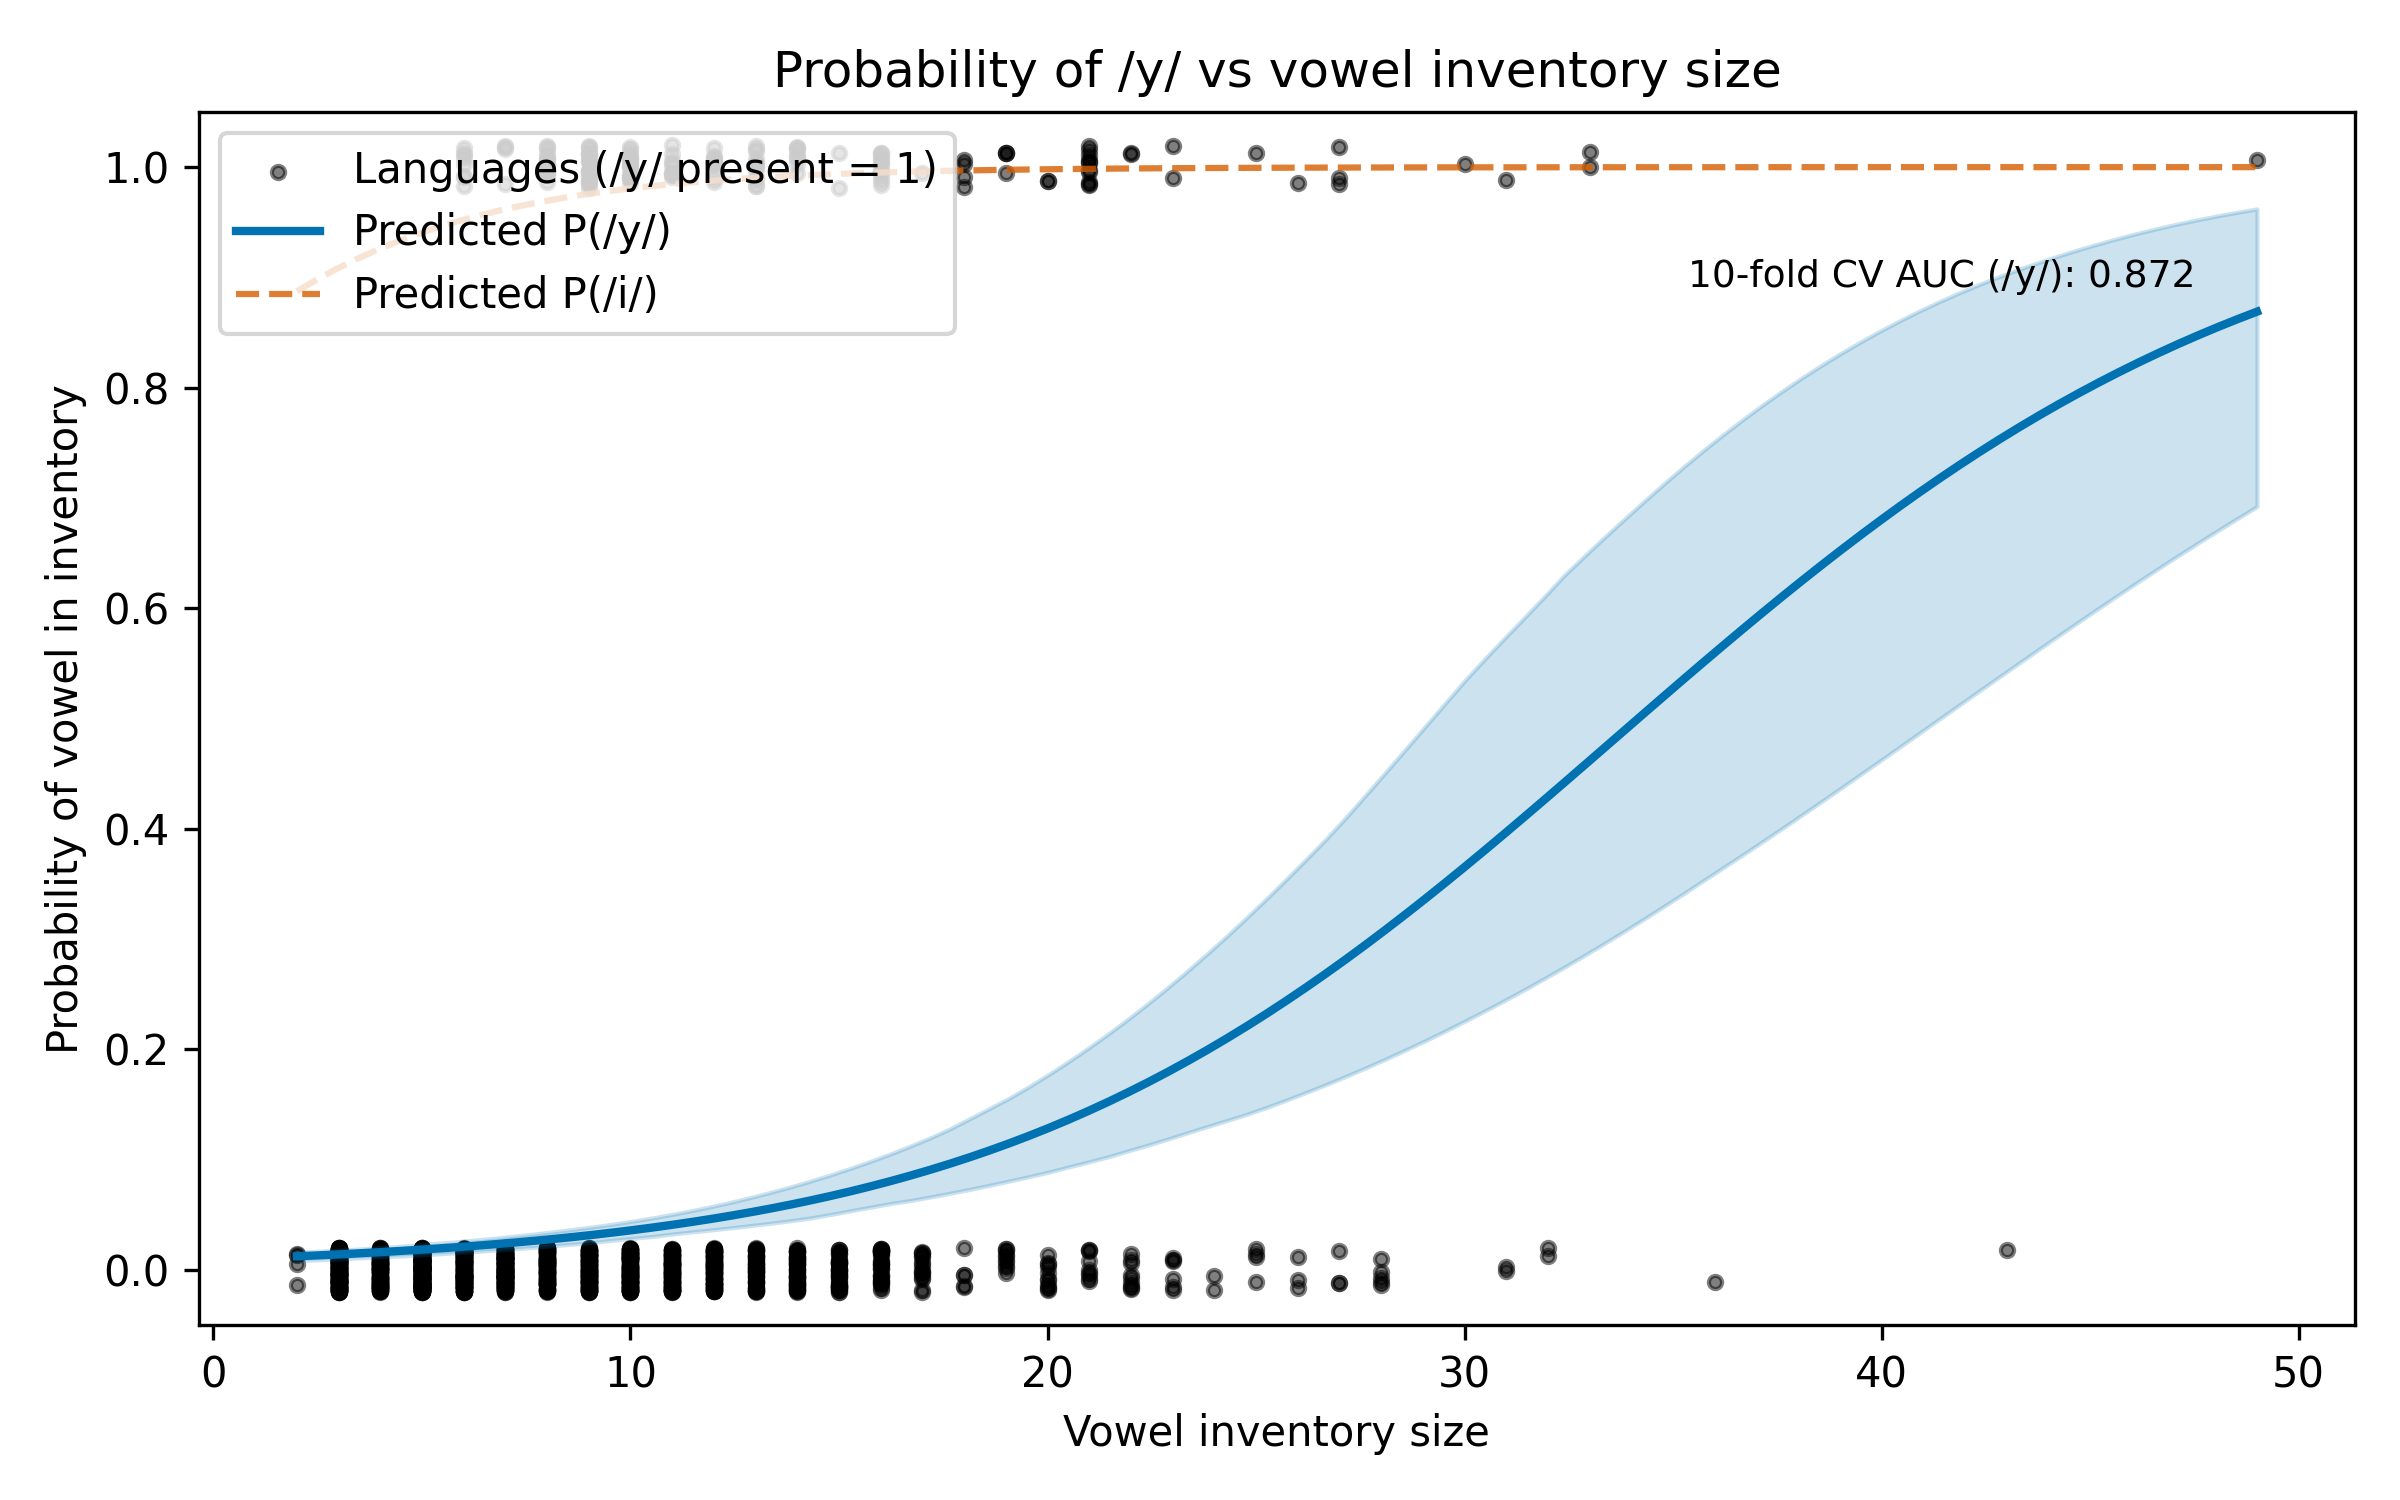
\includegraphics[width=\linewidth]{images/y_vs_vowel_inventory.png}
  \caption{Presence of /\textipa{y}/ as a function of vowel-inventory size.
  Solid line: logistic fit with 95\% CI ribbons; dashed line: comparison curve for /\textipa{i}/.
  Points are languages jittered vertically at 0/1 for presence/absence.
  Model includes a language-family effect; 10-fold cross-validation AUC is shown in-plot.
  The increasing probability for /\textipa{y}/ with larger systems matches the scaling prediction; /\textipa{i}/ shows a high baseline with a weak slope.}
  \label{fig:y-scaling}
\end{figure}

These two results satisfy the \textsc{projectibility} diagnostic in different ways: the ridgelines constrain where inventories fall by family, and the /y/ model supports a scaling inference about specific segments as systems expand. They also have a plausible \textsc{homeostatic} basis. Quantal regions make some vowels (notably /i a u/) robust to articulatory imprecision \citep{Stevens1989Quantal}, dispersion spreads categories for distinctiveness \citep{LiljencrantsLindblom1972,Lindblom1990HandH}, and learning and control bind cues within categories (prototype attraction, audio–motor calibration), while local performance standards and literacy practices stabilise inventories across generations. The cognitive-tool synthesis documents these mechanisms and their empirical signatures \citep[Fig.\,1; Fig.\,2; Table~1]{Ekstrom2025PhonemeTool}. Read together, they explain why families share a stability band and why /y/ appears mainly in larger vowel systems.

Obvious worries are addressable. Counting conventions can inflate tails; excluding tones and prosodies eliminates that source. Genealogical non-independence can spuriously sharpen slopes; modelling a family effect and balancing folds by family leaves the inference intact. Orthographic noise can misclassify vowels; the repository records Unicode normalization and diacritic handling. None of these considerations undermines the main point: phoneme inventories exhibit projectible structure underwritten by concrete stabilizers, and so qualify as \textsc{HPC} kinds at the population–time scales analysed here.



\clearpage
\bibliographystyle{apalike}
\bibliography{refs}

\end{document}
